\subsection{Video}
Das Video Model, enthält zum einen alle Metadaten eines Videos und zum anderen statische Methoden um auf eine bestimmte Anzahl Videos zuzugreifen, sowie Kommentare, Ratings und Videos hinzuzufügen.
\begin{figure}[h!]
\centering
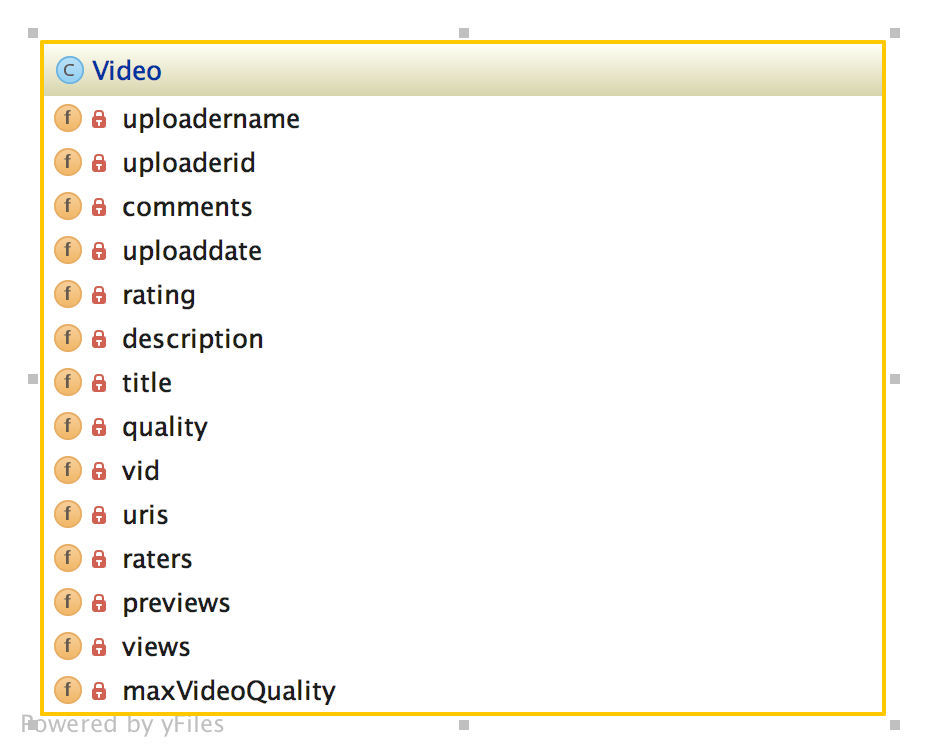
\includegraphics[width=0.7\textwidth]{./UML/VideoMeta.png}
\caption{Metadaten eines Videos}
\end{figure}
\clearpage
Beim erstellen eines Video Objektes durch übergeben einer ID wird durch den Konstruktor der Klasse automatisch alle Metadaten durch ein REST-Call gesetzt.
\begin{lstlisting}[language=php]
public function __construct($id){
            $ret = json_decode(RestAPI::get("/videos/".$id,array("id" => $id)));

            if (isset($ret->error)){
                Controller::redirect("/404");
            }
            else{
                $this->views = $ret->views;
                $this->vid = $ret->id;
                $this->title = (empty($ret->title) ? 'Kein Titel' : $ret->title);
                $this->description = $ret->description;
                $this->uploaderid = $ret->uploaderid;
                $this->uploadername = $ret->uploadername;
                $this->uploaddate = $ret->uploaddate;
                $this->rating = (empty($ret->rating) ? 0 : $ret->rating);
                $this->uris = $ret->uri;
                $this->previews = $ret->previews;
                $this->comments = $ret->comments;
                $this->raters = $ret->ratings->items;
                $this->maxVideoQuality = $ret->maxVideoQuality;
            }

        }
\end{lstlisting}
Das sind alle Metadaten die der Backend Server liefert. \pm
\begin{figure}[h!]
\centering
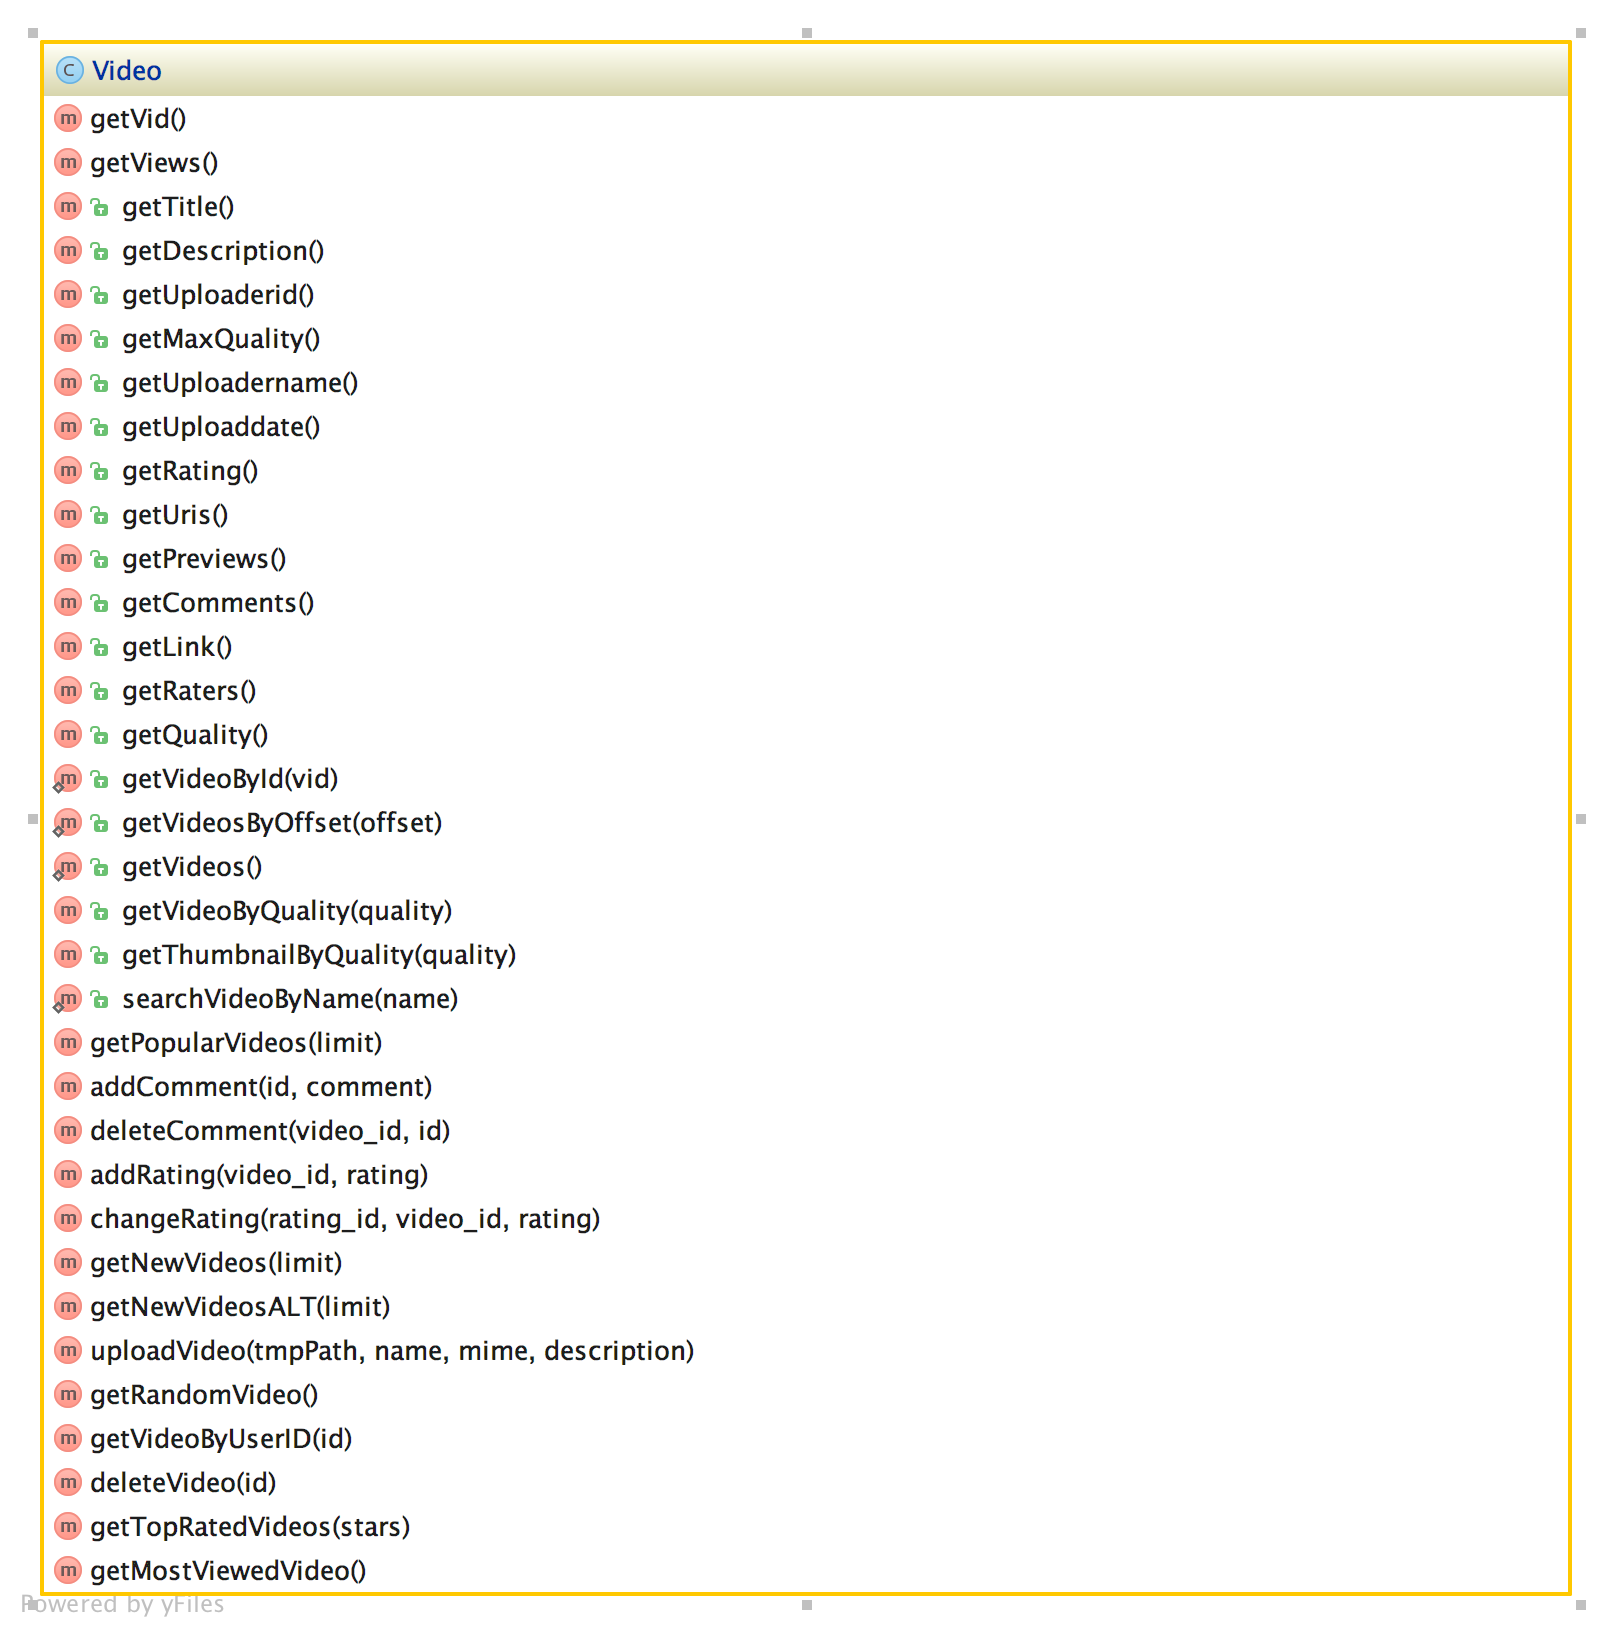
\includegraphics[width=0.7\textwidth]{./UML/VideoFunction.png}
\caption{Funktionen der Video Klasse}
\end{figure}
Neben den trivialen Getter Methoden wird in der Video Klasse noch Funktionalitäten rund um das Video als statische Methoden implementiert.\\
\texttt{getTopRatedVideos, getRandomVideo, getNewVideos, getVideoByUserID} und \texttt{getPopularVideos} geben durch gezielte Suche bestimmte Arten von Videos zurück.\\
\texttt{addComment,deleteComment,addRating, uploadVideo, deleteVideo, searchVideoByName} und \texttt{changeRating} stehen als Schnittstellen zwischen ihren jeweiligen AJAX Implementationen und dem Backend.\\
\begin{lstlisting}[language=php,caption=Examplarische Implementation einer Methode des Video Models]
public static function getPopularVideos($limit){
        $ret = RestAPI::get("/search?type=popularvideos&limit=" . $limit); //REST Call
        return json_decode($ret);//Als PHP JSON (stdClass) Objekt zurückgeben
	}
\end{lstlisting} 
\tb{Anmerkung:} Die Klassenstruktur und die nicht statischen Methoden wurden von Finn Ickler implementiert. Die statischen Methoden vom Rest des Teams.